\chapter{Suchalgorithmen}
\section{Systematische Suche}
Ein rationaler Agent sieht die Welt in verschiedenen Stati, z.B. wären da der aktuelle Zustand und der Zielzustand der Welt. Der rationale Agent muss jetzt eine Folge von Aktionen finden, welche ihn vom Initialzustand in den Zielzustand bringt.
\subsection{Voraussetzungen für eine Suche}
Ein rationaler Agent ist in den Ferien und muss so schnell wie möglich von Arad nach Bukarest , da dort sein Flieger geht. Wie schafft er das? Mit der Suche eines schnellstmöglichen Weges. \\ \newline
Generell kann man sagen, dass wenn die Umwelt folgende Eigenschaften erfüllt, der Agent eine \textbf{Sequenz von Aktionen} suchen kann, welche ihn zum Zielzustand führen werden:

\begin{enumerate}
	\item \textbf{Observable} - Der Agent weiss, wo er ist.
	\item \textbf{Static} - Die Umwelt verändert sich nicht plötzlich.
	\item \textbf{Deterministic} - Jede Aktion hat den gewünschten Effekt.
	\item \textbf{Discrete} - Nur eine finite Anzahl von Aktionen ist möglich in jedem Zustand.
\end{enumerate}

Im Beispiel Arad nach Bukarest sind diese Eigenschaften gegeben. Der Agent weiss, wo er sich befindet, die Städte verändern nicht plötzlich den Ort, und wenn er von einer Stadt in die nächste fährt, dann fährt er auch dorthin. Und, gegeben die Abstraktion, er kann nicht unendlich viele Städte direkt erreichen. Ein Status wäre hier z.B. die aktuelle Stadt auf der Karte, die Aktionen die Reise zwischen den Städten - also die Kanten des Graphen, die Aktionskosten die Distanz-Informationen auf den Kanten. 

\begin{figure}[h]
\centering
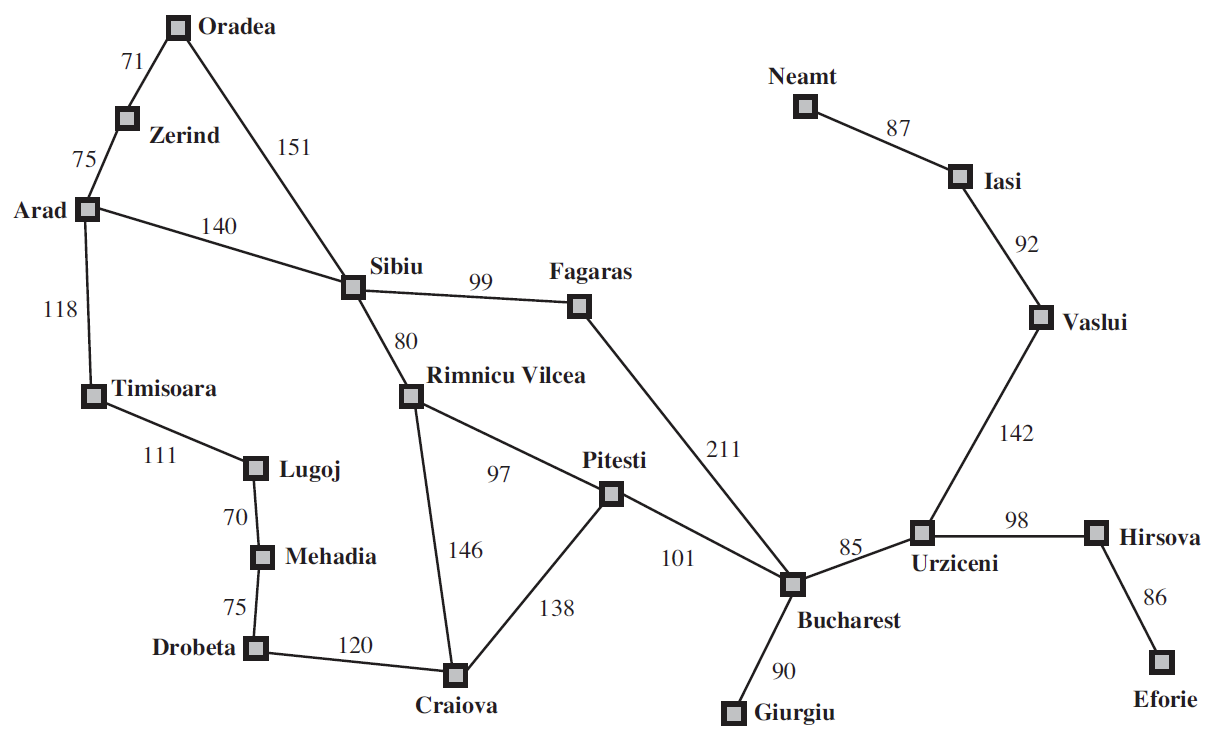
\includegraphics[width=0.5\linewidth]{fig/travel_example}
\caption{Beispiel für eine Umgebung wo eine Suche möglich ist}
\label{fig:travel_example}
\end{figure}

\subsection{Begrifflichkeiten}
\begin{description}
	\item[Initial State] Der erste Status des Agenten
	\item[State Space] Alle möglichen Stati (z.B. der Graph aller Städte)
	\item[Actions] Alle möglichen Aktionen
	\item[Transition Model] Eine Funktion, welche as Input einen Status und eine Aktion hat, und daraus einen neuen Status generiert. z.B. \texttt{succ(Arad, (Arad-Sibiu)) = Sibiu}.
	\item[Goal Test] Sind wir schon da? Sind wir schon da?
	\item[Path] Die Sequenz der Aktionen.
	\item[Path Costs] Die Kostenfunktion über den Gesamtpfad. Meistens die Summe der Kosten aller Einzelaktionen, aber z.B. bei einer Aktion 3 für 2 wäre es wieder anders.
	\item[Solution] Pfad vom Intialzustand zum Zielzustand.
	\item[Optimal Solution] Pfad vom Initialzustand zum Zielzustand mit den niedrigsten Kosten.
	\item[Search Costs] Die Kosten (Zeit \& Speicherverbrauch) um eine Lösung zu finden.
\end{description}

\subsection{Beispielmodelle}
\subsubsection{8 Puzzle}
\begin{figure}[h!]
\centering
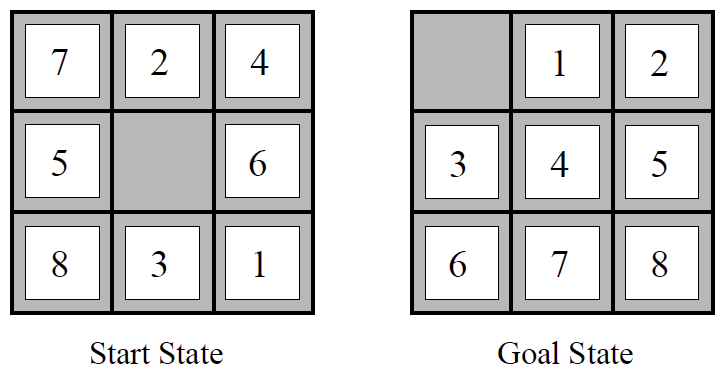
\includegraphics[width=0.6\linewidth]{fig/8_puzzle}
\caption{Das Spiel 8 Puzzle}
\label{fig:8puzzle}
\end{figure}

In diesem Spiel wäre der aktuelle Status die Position der Spielsteine. Die Aktionen wären \textit{bewege das leere Feld} (simpler als die anderen zu bewegen) und der Goal Test wäre dann einfach \textit{ist der Zielzustand = aktueller Zustand}. Die Pfadkosten, sind hier definiert als jede Aktion kostet 1.

\subsubsection{8 Queens}
In diesem Spiel geht es darum, 8 Damen auf einem Feld so zu platzieren, dass keine Dame eine andere Dame bedroht. Hier ist der Zielzustand im Vorfeld unbekannt.
\begin{figure}[h!]
	\centering
	\begin{subfigure}[h]{0.2\textwidth}
	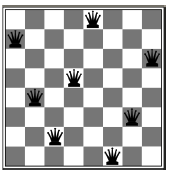
\includegraphics[width=\textwidth]{fig/8_queens_end}
		\caption{Zielzustand 1}
	\end{subfigure}
	~
	\begin{subfigure}[h]{0.2\textwidth}
	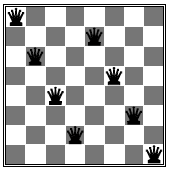
\includegraphics[width=\textwidth]{fig/8_queens_start}
		\caption{Zielzustand 2}
	\end{subfigure}
	\caption{Mögliche Zielzustände}
\end{figure} 

Der aktuelle Status wäre wieder die Position der Damen auf dem Brett, der Initialstatus wäre ein leeres Brett, die \textit{Successor function}, dass man eine Dame zum Brett hinzufügt, und der Goal Test ist auch klar - es sind 8 Damen auf dem Brett die sich nicht bedrohen. Die Pfadkosten sind hier eigentlich egal, wir sind ja nur an der Lösung interessiert.

Optimaler wäre die Sucessor Function so zu definieren, dass man die Damen einfach Spaltenweise hinzufügt.

\subsection{Suchbaum}
\begin{figure}[h!]
	\centering
	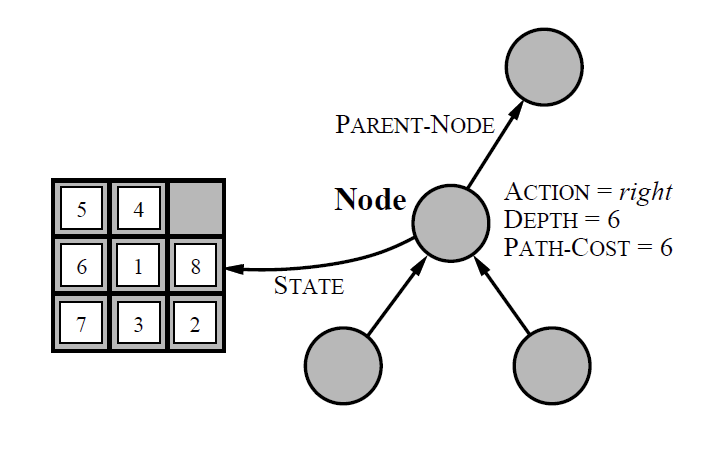
\includegraphics[width=0.5\linewidth]{fig/search_tree}
	\caption{Suchbaum Aufbau}
	\label{fig:search_tree}
\end{figure}
Ein Suchbaum beschreibt die Reihenfolge, in der Knoten im Suchraum besucht werden. Ein Knoten beschreibt dabei einen Status, die letzte Aktion, die zu ihm geführt hat (denn Status + Aktion = Status) und die aktuellen Pfadkosten. Er hat verschiedene Kinder, welche durch entsprechende Aktionen erreicht werden können.
\begin{description}
	\item[Frontier] Die Knoten, welche gerade von der Suchfunktion gefunden wurden und die noch nicht weiter untersucht werden.
	\item[Repeated State] Stati, welche im aktuellen Suchbaum schonmal vorkamen.
	\item[Redundant Paths] Wenn 2 Pfade gefunden werden, welche zum selben Status gelangen.
	\item[Search Space] = Suchraum. Ein Graph, indem die Knoten alle Stati im \textit{State Space} darstellen und die durch entsprechende Aktionen verbunden sind.
	\item[Node expansion] Generiert alle Nachfolge-Knoten, gegeben die Aktionen.
	\item[Search Strategy] Bestimmt, welcher Knoten als nächstes expandiert / exploriert wird.
	\item[Tree-based Search] Suche bei der nur die Frontier gespeichert wird und die bereits besuchte Knoten immer wieder besuchen kann.
	\item[Graph-based Search] Suche bei der zusätzlich die besuchten Knoten ebenfalls gespeichert werden.
	\item[Dead End] Wenn bei einem Knoten keine unbekannten Kinder mehr vorhanden sind.
	\item[Explored Set] Ein Set aus besuchten Knoten. Wird nicht benötigt, wenn der Suchraum keine Schleifen enthält.
\end{description}

\subsection{Suchraum}
\begin{figure} [h!]
	\centering
	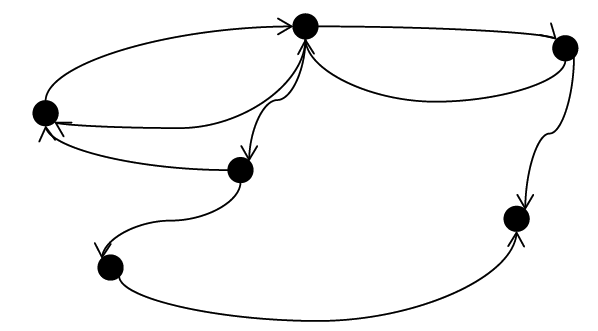
\includegraphics[width=0.2\linewidth]{fig/search_space}
	\caption{Beispiel für Suchraum 1}
	\label{fig:search_space}
\end{figure}

\begin{figure} [h!]
	\centering
	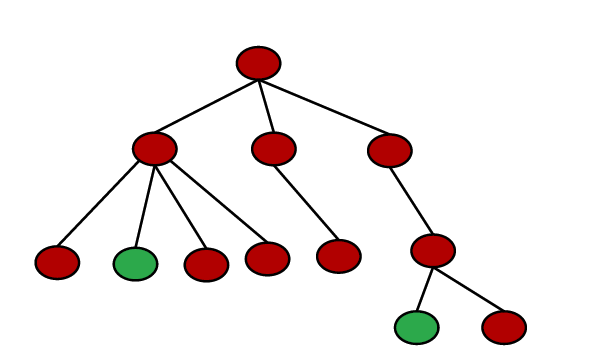
\includegraphics[width=0.2\linewidth]{fig/suchraum}
	\caption{Beispiel für Suchraum 2}
	\label{fig:suchraum}
\end{figure}

Dieser Suchraum in Abbildung \ref{fig:suchraum} hat bestimmte Eigenschaften.
\begin{description}
	\item[b] Branching Factor - max. Anzahl Kinder eines Knotens - hier \textbf{4}
	\item[d] Depth of shallowest goal - hier wäre die Tiefe des ersten grünen Knotens \textbf{2}.
	\item[m] Maximum Length - Maximale Pfadlänge - hier \textbf{3}.
\end{description}

\subsection{Breadth-First Search (BFS)}
Hier wird zuerst in die Breite gesucht. Das heisst, dass wenn ein Knoten gefunden wird, wird er in eine FIFO Queue gesteckt, welche dann nacheinander abgearbeitet wird.
\begin{figure} [h!]
	\centering
	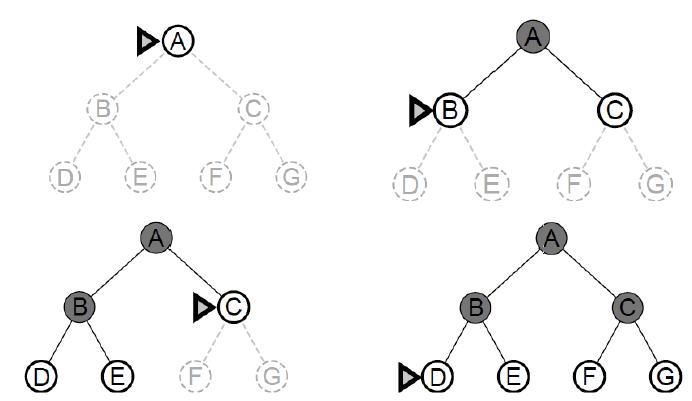
\includegraphics[width=0.4\linewidth]{fig/bfs_search}
	\caption{Breadth-First Search}
	\label{fig:bfs}
\end{figure}
BFS findet alle Lösungen und wenn die Aktionen alle dieselben positiven (oder null) Kosten haben, dann findet es auch die optimale Lösung. Es findet ja immer die Lösung, die am wenigsten tief im Baum vorhanden ist.
\subsubsection{Zeitbedarf \& Zeitkomplexität}
Ein BFS Suchbaum muss ja bis zur Tiefe des Lösungsobjekt komplett aufgebaut werden. Wenn \textbf{b} der \textit{branching factor} ist und \textbf{d} die Tiefe der Lösung heisst das, dass diese Anzahl an Knoten besucht werden müssen:

\begin{displaymath}
	\displaystyle\sum_{i=1}^{d} b^i = b + b^2 + b^3 + \dots + b^d \approx O(b^d)
\end{displaymath}

\subsubsection{Speicherbedarf \& Speicherkomplexität}
BFS speichert offenbar jeden besuchten Knoten ab, da der Pfad zur gefundenen Lösung ja auch bekannt sein muss. Daher ist der Speicherbedarf, gleich wie der Zeitbedarf:

\begin{displaymath}
\displaystyle\sum_{i=1}^{d} b^i = b + b^2 + b^3 + \dots + b^d \approx O(b^d)
\end{displaymath}
Die Frontier hat \(O(b^d)\) und das explored set \(O(b^{d-1})\).

\subsection{Depth-First Search (DFS)}
Die Depth First Search ist ähnlich wie die Breadth-First Search. Die gefundenen Knoten werden hier aber in eine LIFO Queue gesteckt. Das bewirkt, dass zuerst in die Tiefe gesucht wird und erst dann schrittweise in die Breite.
\begin{figure} [h!]
	\centering
	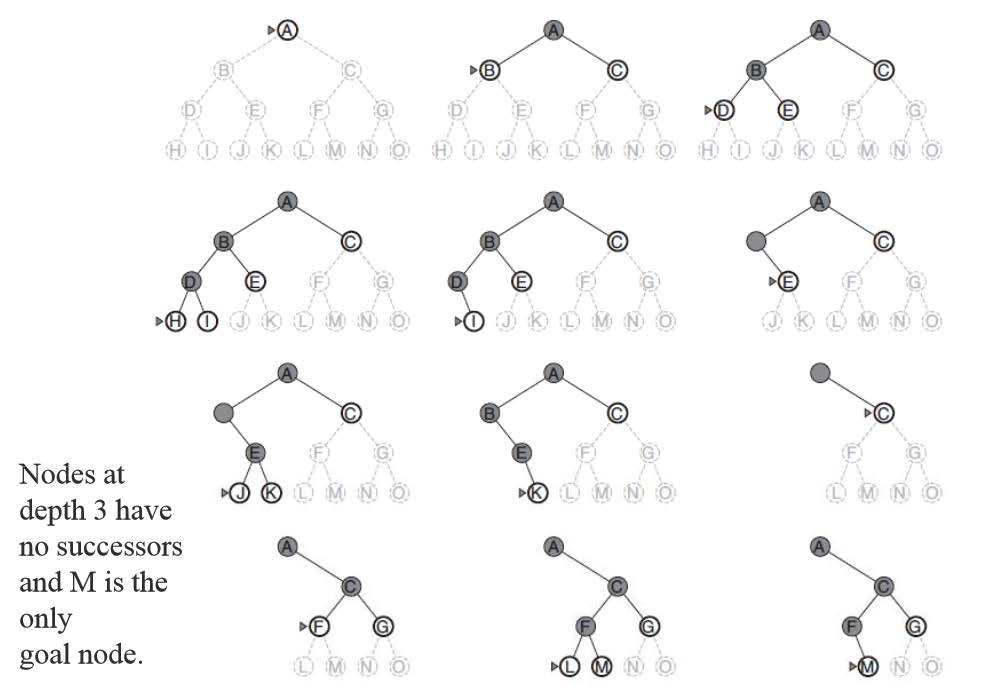
\includegraphics[width=0.7\linewidth]{fig/dfs_search}
	\caption{Depth-First Search}
	\label{fig:dfs}
\end{figure}
DFS ist keine optimale Suche, es kann sein dass eine Lösung tief unten 'vergraben' liegt, und wenn sie dann unendlich tief ist, geht sie dort natürlich auch suchen. Wenn die besuchten Knoten zusätzlich nicht gespeichert werden, dann kann sie auch für immer im Kreis herum suchen.
\subsubsection{Zeitbedarf \& Zeitkomplexität}
Eine DFS Suche findet im schlechtesten Fall die Lösung erst wenn der ganze Baum durchsucht wurde. \textbf{m} heisst ja die maximale Tiefe und \textbf{b} wieder der \textit{branching factor.}

\begin{displaymath}
	b^m \approx O(b^m)
\end{displaymath}

\subsubsection{Speicherbedarf \& Speicheromplexität}
DFS muss nicht der gesamte Baum speichern, sondern nur der Pfad der gerade zum Objekt führt.

\begin{displaymath}
bm \approx O(bm)
\end{displaymath}
In Abbildung \ref{fig:dfs} sieht man das schön. Dort hat der Baum \(b=2, m=3\). In keinem Fall müssen also mehr als \(2*3=6\) Knoten gespeichert werden. \\ \newline
Wenn der Suchraum allerdings noch Schlaufen beinhaltet, so muss noch die besuchten Knoten gespeichert werden. Das kann bedeuten, dass im schlechtesten Fall der gesamte Baum abgespeichert werden muss.

\begin{displaymath}
b^m \approx O(b^m)
\end{displaymath}

\subsection{Depth-Limited Search (DLS)}
DLS ist DFS, einfach mit einem Limit wie tief die Suche gehen darf. Läuft jetzt nicht mehr unendlich, aber wenn die Lösung tiefer ist als das Limit wird sie natürlich nicht gefunden.
\subsubsection{Zeitbedarf \& Zeitkomplexität}
Gleich wie DFS, einfach anstatt Tiefe des Baums die Tiefe des Suchlimits. Das heisst Zeitbedarf ist jetzt (\textbf{l} = Limit)
\begin{displaymath}
b^l \approx O(b^l)
\end{displaymath}
\subsubsection{Speicherbedarf \& Speicheromplexität}
... und Speicherbedarf:
\begin{displaymath}
bl \approx O(bl)
\end{displaymath}

\subsection{Iterative Deepening Search (IDS)}
Wie DLS, einfach wird das Limit schrittweise angehoben. Ist also irgendwie eine Mischung aus BFS und DFS. Die ersten Schritte der Suche werden immer wiederholt, was aber sich aber nicht auf die Gesamtkomplexität auswirkt. Es findet immer eine Lösung wenn eine da ist und ist sogar optimal, wenn die Kostenfunktion nicht abnimmt mit der Tiefe des Suchbaums.

\subsubsection{Zeitbedarf \& Zeitkomplexität}
Komplexität gleich wie DLS / DFS, einfach anstatt Limit wieder der Gesamte Baum. Aber der echte Zeitbedarf ist etwas grösser, da ja jeder Knoten besucht wird.
\begin{displaymath}
	(d)b+(d-1)b^2+\dots +3b^{d-2}+2b^{d-1}+1b^{d} \approx O(b^d)
\end{displaymath}
\subsubsection{Speicherbedarf \& Speicheromplexität}
... und Speicherbedarf ebenfalls:
\begin{displaymath}
	bd \approx O(bd)
\end{displaymath}

\subsection{Uniform Cost Search (UCS)}
Hier werden wieder die Nodes analog DFS und BFS gefunden. Die Queue hier ist aber keine FIFO oder LIFO, sondern eine \textbf{Priority Queue}. Das heisst, dass die gefundenen Nodes anhand ihrer bisherigen \textbf{Gesamt-Pfadkosten} sortiert werden und zuerst die Knoten expandiert werden, welche die geringsten Kosten haben. So findet UCS die optimale Lösung, sofern die Nachfolgeknoten immer grössere Gesamtkosten haben als der aktuelle Knoten.\\ \newline
Wichtig bei der Implementation wäre noch, dass nicht beim Finden, resp. expandieren der Frontier getestet wird, ob dies ein Zielknoten ist, sondern erst, wenn der nächste Knoten aus der sortierten Queue genommen wird. Ansonsten wäre das Resultat wieder nicht optimal. Zudem wird, wenn ein Knoten gefunden wird mit niedrigeren Kosten als derselbe Knoten hat, der in der Frontier vorkommt, dieser in der Frontier ersetzt.\\ \newline
Wenn ein Pfad 0 oder weniger Kostet und unendliche tief runter geht, dann bleibt UCS dort stecken, weil es wirklich nur die Kosten anschaut.

\subsubsection{Zeit- \& Speicherkomplexität}
\begin{displaymath}
O(b^{d+1})  \textrm{ wenn alle Aktionskosten identisch sind}
\end{displaymath}
\begin{displaymath}
O(b^{1+\left\lfloor{o/c}\right \rfloor })  \textrm{ wenn sie nicht identisch sind. o = Kosten optimale Lösung, c = minimale Kosten einer Aktion}.
\end{displaymath}


\subsection{Fragen}
\subsubsection{By which means are search problems formulated?}
\begin{enumerate}
	\item Zielzustand formulieren
	\item Zustandsraum definieren
	\item Mögliche Aktionen festlegen
	\item Suchkosten - suche ich unendlich lange oder mache ich mal
	\item Aktionskosten - Pfadkosten
\end{enumerate}
\subsubsection{How can search problems differ in the characteristics of actions and states?}
Search problems can habe different sets of actions and states. The way the problem is modeled decides.
\subsubsection{Which properties are used to characterize a search method?}
Completeness, Time and Space Complexity and optimality.
\subsubsection{Can you explain how BFS, DFS, DLS, IDS, UCS work?}
See above.
\subsubsection{Compare the 5 uninformed search methods wrt. time complexity, space complexity, optimality, completeness}
See above.

\section{Heuristic (informed) search}
Die uninformierte Suche nimmt einfach irgendwelche Knoten und sucht bei diesen weiter. Bei der informierten, heuristischen, Suche werden den Knoten (Schätz-) Werte zugewiesen, durch eine evaluierungsfunktion \(f(n)\).
\begin{displaymath}
f(n) = g(n) + h(n)
\end{displaymath}
Wobei \(g(n)\) die Kosten vom Erstzustand bis zum aktuellen Zustand und \(h(n)\) die geschätzten Kosten bis zum Ziel sind. \(h(n)\) ist hierbei die \textit{Heuristik}.

\subsection{Eigenschaften von h(n)}\label{sec:heuristic_properties}
\begin{enumerate}
	\item \(h(n) = 0\) wenn \(n\) ein Zielzustand ist.
	\item \(h(n)\) ist \textbf{admissible}. \\
		Es muss die realen Kosten bis zum Ziel unterschätzen.
	\item \(h(n)\) ist \textbf{constistent}\\
		Vom Knoten \(n\) wären es \(\approx\) 10 bis ins Ziel. Zum Nachfolgeknoten \(n'\) kostet es 1. Dann darf der Nachfolgeknoten \(n'\) nicht plötzlich  weniger als \(\approx\) 9 haben.
\end{enumerate}

\subsection{Greedy Search}
Greedy Search verwendet ausschliesslich die Heuristik, um den Weg ins Ziel zu finden. Es garantiert keine optimale Lösung und auch nicht, dass es überhaupt eine Lösung findet. Im Beispiel mit dem Weg von Sibiu nach Bukarest würde es immer den Knoten wählen, der näher bei Bukarest ist als die anderen.

\subsection{A* Search}
A* benutzt die vergangenen Kosten \(g(n))\) und die geschätzten nachfolgenden Kosten \(h(n)\)) und verwendet das als Sortierung für den als nächstes zu evaluierenden Knoten, verwendet also \(f(n)\).
\begin{displaymath}
f(n) = g(n) + h(n)
\end{displaymath}
 Es ist garantiert, dass wenn es eine Lösung gibt, dass A* diese findet, sofern die Heuristik die Eigenschaften von \ref{sec:heuristic_properties} erfüllt. Zudem ist die gefundene Lösung optimal. Der Nachteil ist aber, dass die Zeit- und Speicherkomplexität exponentiell wachsen. Das heisst, dass alles von der gewählten Heuristik abhängt.
 
 \subsection{Beam Search}
Beam Search baut einen Breadt-First Suchbaum auf, aber speichert in jedem Schritt davon nur die \textit{n}-besten und evaluiert danach auch nur diese. \textit{n} ist dabei die \textit{Beamwidth}.  Ist offensichtlich nicht komplett und auch nicht optimal, aber in der Praxis trotzdem manchmal nützlich, wenn der Suchraum riesig ist.
 
 \subsection{IDA*}
IDA* sucht zuerst in die Tiefe und bricht aber ab, wenn die geschätzten Kosten einen gewissen Schwellenwert überschreiten.
 
 \subsection{Branch and Bound}
 Sind mehrere Lösungen gesucht, so kann wenn eine Lösung gefunden wurde, können alle Knoten die höhere Kosten haben, weggeschnitten werden. Denn die Heuristik unterschätzt die Kosten ja immer, dann kann das gar keine gute Lösung mehr werden.
 
 \subsection{Heuristiken}
 \begin{quote}
 	I don't know! - Make an educated guess! --- Oliver Töngi, always.
 \end{quote}
 Das ist eine Heuristik. Eine gute Heuristik, ist informiert (und daher spezifisch) über das Problem.
 \subsubsection{Manhattan Distance}
 Für das 8 Puzzle, siehe Abbildung \ref{fig:8puzzle}, könnten z.B. die Distanzen der falsch platzierten Steine zu ihrer richtigen Position eine Heuristik darstellen. Das wäre die Manhatten Distance (weil Manhattan ja so schachbrettartig aufgebaut ist, dass man sagen kann \textit{zwei Blocks entfernt}).
 \subsubsection{Linear Conflict Heuristic} 
 Wenn sich zwei Steine für die Lösung im Weg sind, also mehr Moves gemacht werden müssen als nötig, wird noch extra was dazuberechnet.
 \subsubsection{Pattern Database}
 Man kann z.B. Teillösungen schon vorausberechnen und wiederverwenden. Für ein grösseres 8 Puzzle z.B. den Rand des Puzzles anhand einer Datenbank bilden und dann der innere Teil erst lösen. Im Schach macht man das auch so, dass man am Ende des Spiels eine vorberechnete Strategie fährt, da dort ja die Zustandsräume nicht mehr so gross sind.
 \subsubsection{Gaschnigs Heuristic}
 Man nehme ein zwei Constraints des Problems weg und suche da eine einfach berechenbare Lösung. z.B. 8 Puzzle als String formatieren und dann schauen, wie aufwändig es ist, das der Reihe nach zu sortieren. Wird häufig gemacht zum noch eine bessere Heuristik herauszufinden. 
 \subsection{Summary Questions}
\subsubsection{Explain the underlying ideas of best-first search, greedy search and beam search.}
Best first search wählt einfach anhand einer Funktion den nächstbesten Knoten zum expandieren aus. Greedy Search ist eine Art von Best First Search und verwendet einfach nur die geschätzten Kosten bis zum Zielpunkt als Evaluation. Beam Search baut einen Breadt-First Suchbaum auf, aber speichert in jedem Schritt davon nur die \textit{n}-besten und evaluiert danach auch nur diese. \textit{n} ist dabei die \textit{Beamwidth}. 
\subsubsection{How do the A* and IDA* algorithms work?}
A* evaluiert die realen, bekannten Kosten bis zu einem Knoten und die geschätzten Kosten bis zum Ziel und wählt immer die besten aus. IDA* macht Tiefensuche, evaluiert dabei 
\subsubsection{What are the principal properties of A*?}
A* needs an admissible and constistent heuristic to work. It requires exponential complexity to solve the problem. 
\subsubsection{Why is IDA* more efficient in practice?}
It doesn't need exponential memory to work.
\subsubsection{What is the principal idea behind branch and bound?}
Die Knoten wegschneiden, welche garantiert nicht zur Lösung führen.
\subsubsection{What are heuristics, which role do they play in informed search, and how can we develop good heuristics?}
Heuristics are educated guesses, they help us to direct the search in the search space towards the desired goal state in an efficient manner. Heuristics are often developed with problem relaxation, whereas one or more constraints from the problem are dropped and a solution is found for the easier problem, from which process the distance to the solution with all restrictions can be guessed.
\subsubsection{What is an admissible heuristics?}
A heuristic which underestimates the real costs to the goal state.
\subsubsection{What can happen to A* if it is used with a non-admissible heuristic?}
It's guaranteed to find the optimal solution, because the too highly estimated nodes are not further evaluated.